\maketitle


\section{Predicting Bike Station Occupancy}
\subsection{Feature Engineering}
\subsubsection{Selection of Station}
In choosing the stations I was going to use I decided to display them on a map.
This would make it easier to choose stations which would have different behaviour.
I decided to choose station 97 (Kilmainham Gaol) as it is the furthest from the city center.
I also chose station 109 (Buckingham Street) as it is beside Connolly and I assumed it would have drastically different behaviour than my other station.

\begin{figure}[H]
\centering
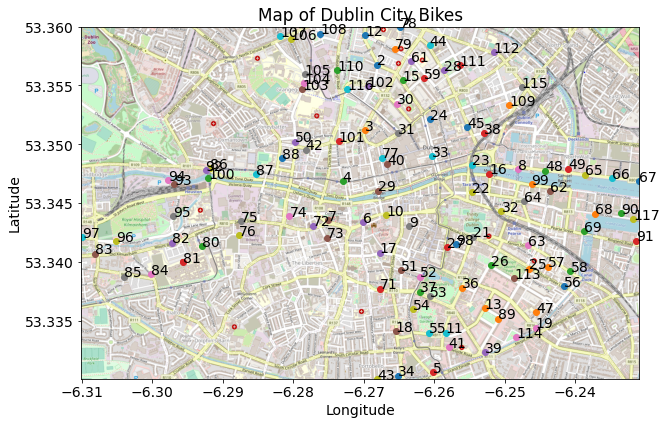
\includegraphics[width=0.5\textwidth]{images/map.png}
\caption{Map of Dublin Bike stations.}
\end{figure}

The data that I needed was the time and number of available bikes.

\begin{figure}[H]
    \centering
    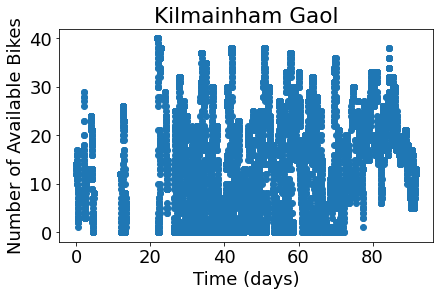
\includegraphics[width=0.5\textwidth]{images/kilmainham data.png}
    \caption{Map of Dublin Bike stations.}
    \end{figure}
\par 

\begin{figure}[H]
    \centering
    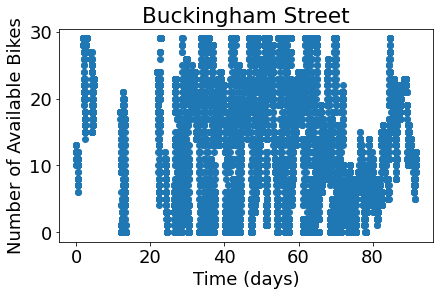
\includegraphics[width=0.5\textwidth]{images/buckingham data.png}
    \caption{Map of Dublin Bike stations.}
    \end{figure}
Much of the data was missing. 
I decided to simply remove the first 27 days in both datasets as 
there was so much missing that it would likely make it more difficult to 
work with the data in a way that didn't negatively affect the performance of the models.
It is likely that there were other missing data points, this is evident in that not every day has the same number of entries (between 287 and 289).
This is unlikey to have any major impact on my predictions as it is very close to 288 
(the number of 5 minute time blocks in a day).



\par 


\subsection{Machine Learning Methodology}
The Machine learning methods I decided to use are\dots
\subsubsection{Method 1}
\subsubsection{Method 2}

\subsection{Evaluation}
\subsubsection{Method 1}
\subsubsection{Method 2}
